\chapter{张量与相对论洛伦兹力}

今晚我们将从标量场转向电动力学。前面的讨论确立了一个有用的模式：一个作用量既描述场如何作用于粒子，也描述粒子如何反作用于场。我们最终会把这一模式应用于电磁场，但首先我们需要足够强的记号来揭示计算的对称性。

这项准备工作并非装饰。一个负号、一个零、一个等号以及矢量记号，各自都压缩了一个否则不得不用文字重复表达的思想。张量记号对相对论也起着同样的作用。一旦上、下指标、缩并和变换律就位，电力和磁力就会自行组装成一个四维方程。

\section{四维矢量与指标的节约}

\subsection{上分量与下分量}

希腊指标遍历全部四个时空坐标，而拉丁指标只遍历三个空间坐标：
\begin{equation}
\mu,\nu,\rho,\sigma=0,1,2,3,
\qquad
m,n=1,2,3.
\end{equation}
一般的逆变四维矢量为 \(A^\mu=(A^0,A^1,A^2,A^3)\)。
按照这里采用的约定，
\begin{equation}
\eta_{\mu\nu}
=
\begin{pmatrix}
-1&0&0&0\\
0&1&0&0\\
0&0&1&0\\
0&0&0&1
\end{pmatrix},
\qquad
A_\mu=\eta_{\mu\nu}A^\nu .
\label{eq:sr6-metric-lowering}
\end{equation}
因此，降下一个指标会改变时间分量的符号，而空间分量保持不变：
\begin{equation}
A_0=-A^0,
\qquad
A_m=A^m.
\label{eq:sr6-component-lowering}
\end{equation}
对于平直时空，这就是该操作的全部内容，尽管同样的记号在广义相对论中会获得更丰富的几何意义。

\begin{figure}[htbp]
\centering
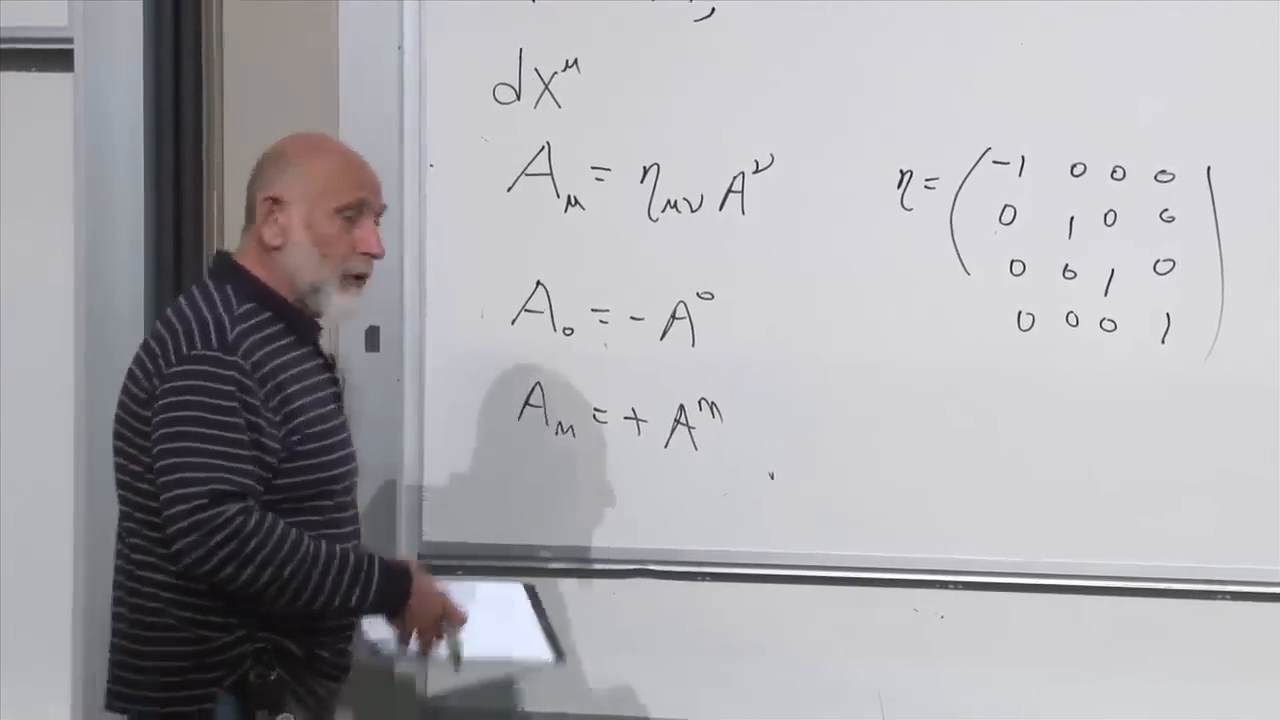
\includegraphics[width=0.90\textwidth]{lecture_06_figure_01.png}
\caption{闵可夫斯基度规以及降下四维矢量指标的份量规则。}
\lectureframe{00:07:45}
\end{figure}

当一个指标在上方出现一次、在下方出现一次时，使用爱因斯坦求和约定。因此缩并
\begin{equation}
A_\mu B^\mu
=
-A^0B^0+A^1B^1+A^2B^2+A^3B^3
\label{eq:sr6-vector-contraction}
\end{equation}
是一个标量。如果某个求和不具有这种上--下重复的形式，我们将显式写出其求和号。

\subsection{导数带有下指标}

四个导数算符被收集为
\begin{equation}
\partial_\mu
\equiv
\frac{\partial}{\partial x^\mu}.
\end{equation}
作用于标量场 \(\phi(x)\) 时，它们构成协变矢量
\(\partial_\mu\phi\)。看出指标位置的最快方式是考虑一个无穷小位移：
\begin{equation}
d\phi
=
\frac{\partial\phi}{\partial x^\mu}\,dx^\mu
=
\partial_\mu\phi\,dx^\mu.
\label{eq:sr6-total-differential}
\end{equation}
左边是相邻事件处标量值之差，因此是一个标量。由于 \(dx^\mu\) 是逆变的，与它缩并的对象必须是协变的。

\begin{classroomqa}
\audiencequestion{如果 \(x^\mu\) 带有上指标，为什么对 \(x^\mu\) 求导会产生下指标？}
\lecturerresponse{因为微分变化 \(d\phi=\partial_\mu\phi\,dx^\mu\) 是一个标量。逆变位移只有与协变梯度缩并才能产生该标量。因此，导数指标的位置由其变换律决定，而不是仅由分式的排版决定。\lecturetimestamp{00:10:10}}
\end{classroomqa}

\begin{figure}[htbp]
\centering
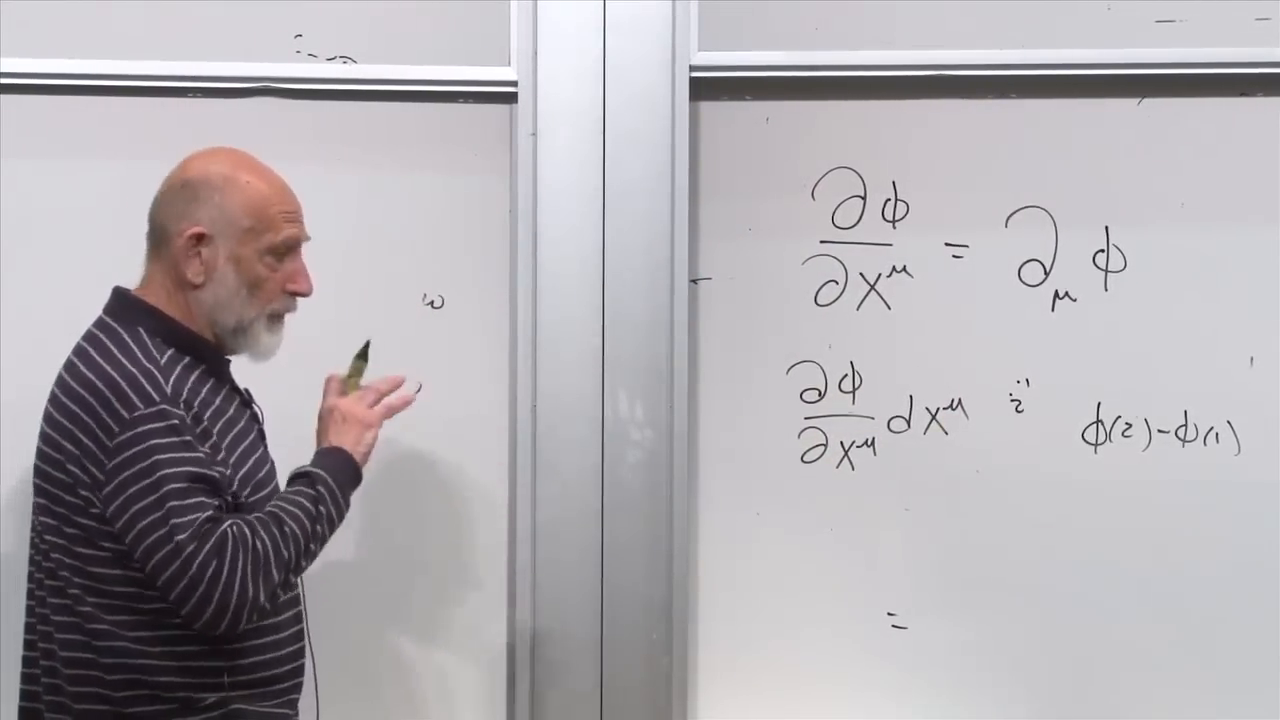
\includegraphics[width=0.90\textwidth]{lecture_06_figure_02.png}
\caption{标量微分 \(d\phi\) 表明 \(\partial_\mu\phi\) 是一个协变矢量。}
\lectureframe{00:11:05}
\end{figure}

同一规则提供了另一个标量。如果 \(B^\mu(x)\) 是一个四维矢量场，那么
\begin{equation}
\partial_\mu B^\mu
\label{eq:sr6-four-divergence}
\end{equation}
就是它的四维散度。它将时间分量的时间导数与相应空间分量的三个空间导数结合在一起。

\begin{figure}[htbp]
\centering
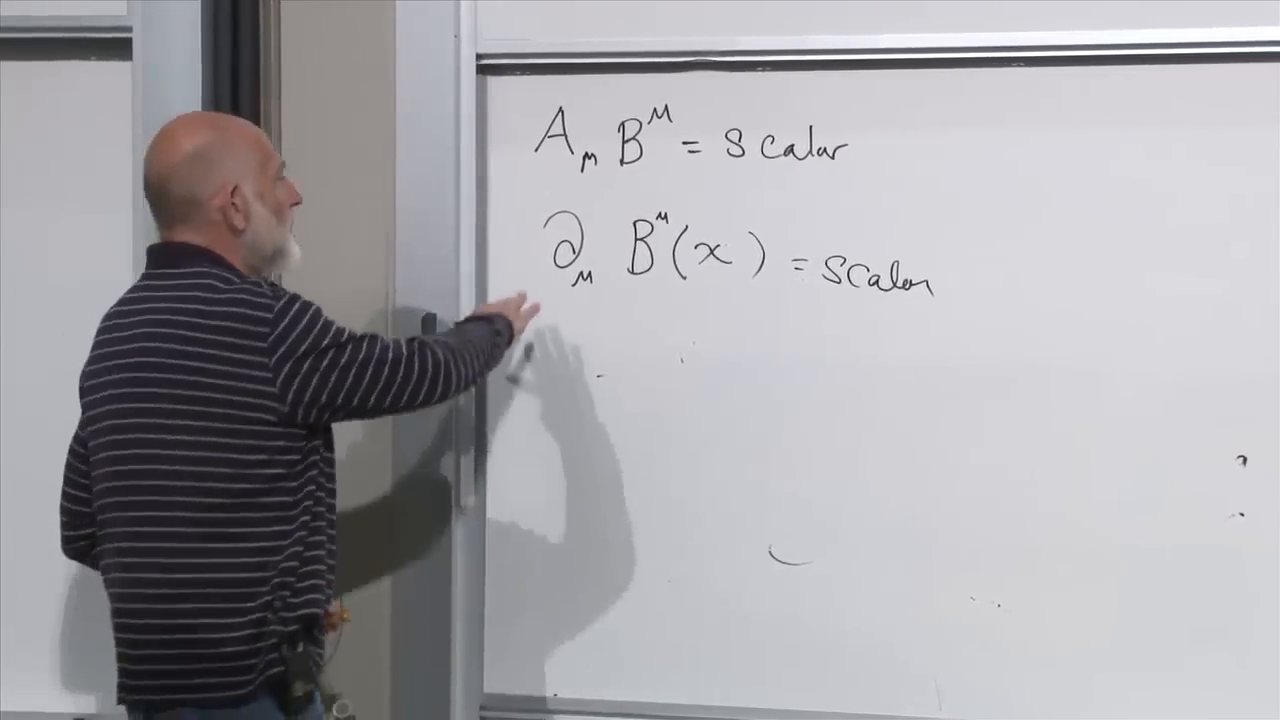
\includegraphics[width=0.90\textwidth]{lecture_06_figure_03.png}
\caption{两个标量缩并：\(A_\mu B^\mu\) 和四维散度 \(\partial_\mu B^\mu(x)\)。}
\lectureframe{00:14:00}
\end{figure}

所有这些都有一个三维类比。在欧几里得三维空间中，度规是单位矩阵，因此升高或降低拉丁指标不改变任何东西。因此，在方便时我们会将空间指标上下移动，同时继续仔细区分时空指标。

\section{矩阵形式的洛伦兹变换}

标量和矢量由它们的变换方式定义。标量保持相同的值，而逆变四维矢量服从
\begin{equation}
(A^\mu)'=L^\mu{}_\nu A^\nu.
\label{eq:sr6-vector-transform}
\end{equation}
可见指标 \(\mu\) 是自由的，并且在两边都出现。重复指标 \(\nu\) 被求和，并从最终的分量方程中消失。

这里 \emph{洛伦兹变换} 既包括空间旋转，也包括助推。助推可以指向任意轴；旋转可以与助推复合以产生一般变换。空间旋转本身不改变时间坐标。

\begin{classroomqa}
\audiencequestion{当我们旋转空间时，时间完全不受影响吗？}
\lecturerresponse{是的。在普通空间旋转中，时间分量不变。这类旋转与混合时间和空间的变换一起被包含在洛伦兹群中。\lecturetimestamp{00:16:27}}
\end{classroomqa}

对于沿 \(x\) 轴、速率为 \(v\) 的助推，其中 \(c=1\)，
\begin{equation}
L^\mu{}_\nu
=
\begin{pmatrix}
\gamma&-\gamma v&0&0\\
-\gamma v&\gamma&0&0\\
0&0&1&0\\
0&0&0&1
\end{pmatrix},
\qquad
\gamma=\frac{1}{\sqrt{1-v^2}}.
\label{eq:sr6-boost-matrix}
\end{equation}
乘以 \((t,x,y,z)^{\mathsf T}\) 得到
\begin{equation}
\begin{aligned}
t'&=\gamma(t-vx),\\
x'&=\gamma(x-vt),\\
y'&=y,\\
z'&=z.
\end{aligned}
\end{equation}
当矩阵在黑板上补全时，该类提供了零和两个单位元。

\begin{figure}[htbp]
\centering
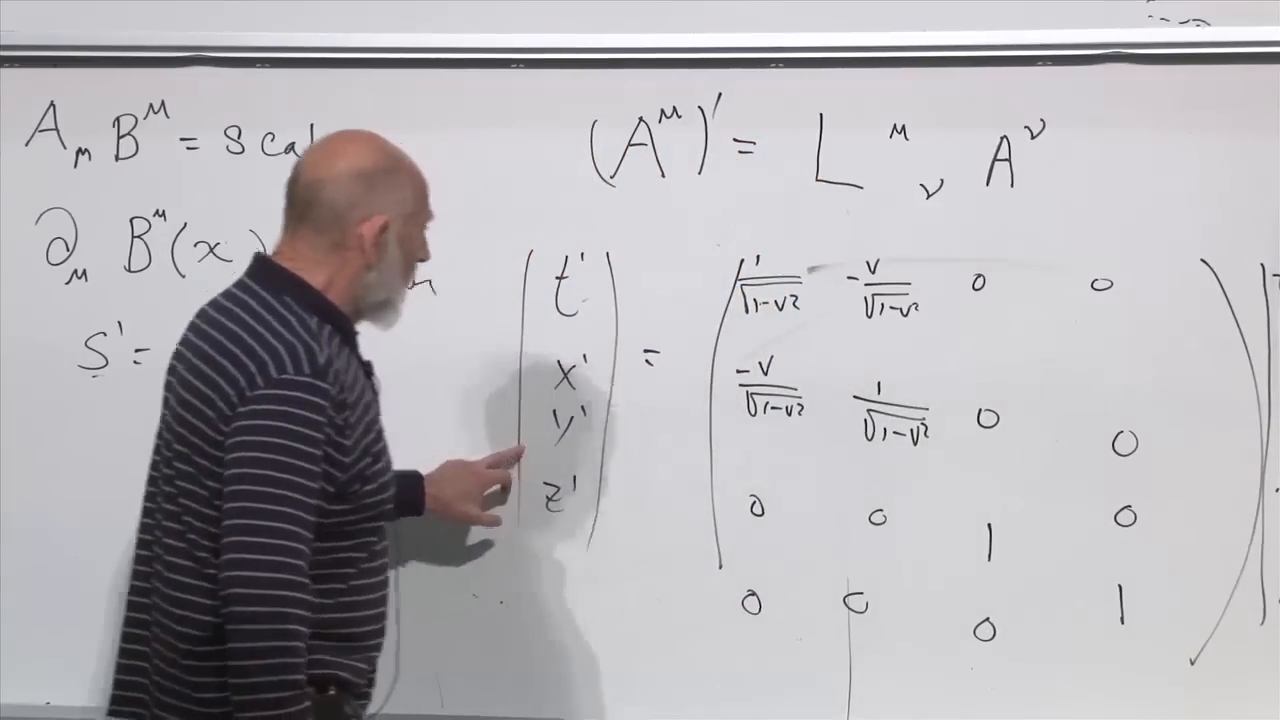
\includegraphics[width=0.90\textwidth]{lecture_06_figure_04.png}
\caption{作用于列\((t,x,y,z)^{\mathsf T}\)的沿\(x\)方向的助推矩阵。}
\lectureframe{00:21:35}
\end{figure}

在\(y\)--\(z\)平面内转过角度\(\theta\)的旋转则给出
\begin{equation}
R_{yz}(\theta)
=
\begin{pmatrix}
1&0&0&0\\
0&1&0&0\\
0&0&\cos\theta&\sin\theta\\
0&0&-\sin\theta&\cos\theta
\end{pmatrix}.
\label{eq:sr6-yz-rotation}
\end{equation}
它表明
\begin{equation}
y'=y\cos\theta+z\sin\theta,
\qquad
z'=-y\sin\theta+z\cos\theta,
\end{equation}
而\(t\)和\(x\)保持不变。诸如
\eqref{eq:sr6-boost-matrix}和\eqref{eq:sr6-yz-rotation}这样的矩阵乘积生成更一般的洛伦兹变换。

\begin{figure}[htbp]
\centering
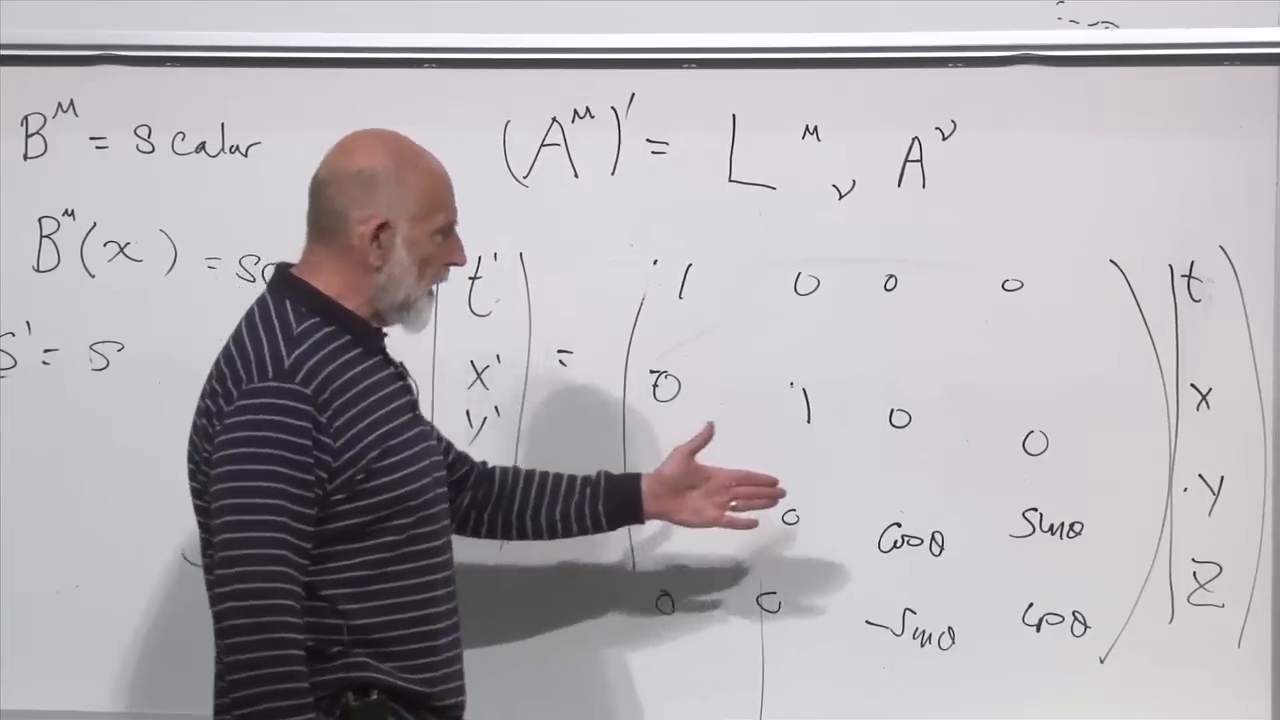
\includegraphics[width=0.90\textwidth]{lecture_06_figure_05.png}
\caption{在\(y\)--\(z\)平面内的纯旋转，其中\(t\)和\(x\)不受影响。}
\lectureframe{00:23:10}
\end{figure}

协变矢量用指标位置相反的矩阵来变换：
\begin{equation}
(A_\mu)'=M_\mu{}^\nu A_\nu.
\label{eq:sr6-covector-transform}
\end{equation}
黑板前的一次听众纠错发现了一个暂时重复的自由指标：左边未求和的\(\mu\)也必须是右边未求和的指标。这两个矩阵表示同一个物理上的参考系变换，它们之间的关系为
\begin{equation}
M=\eta L\eta,
\qquad
\eta^{-1}=\eta.
\label{eq:sr6-M-L-relation}
\end{equation}
最后一个恒等式之所以立即成立，是因为\(\eta\)的每个对角元都是其自身的逆。

\begin{figure}[htbp]
\centering
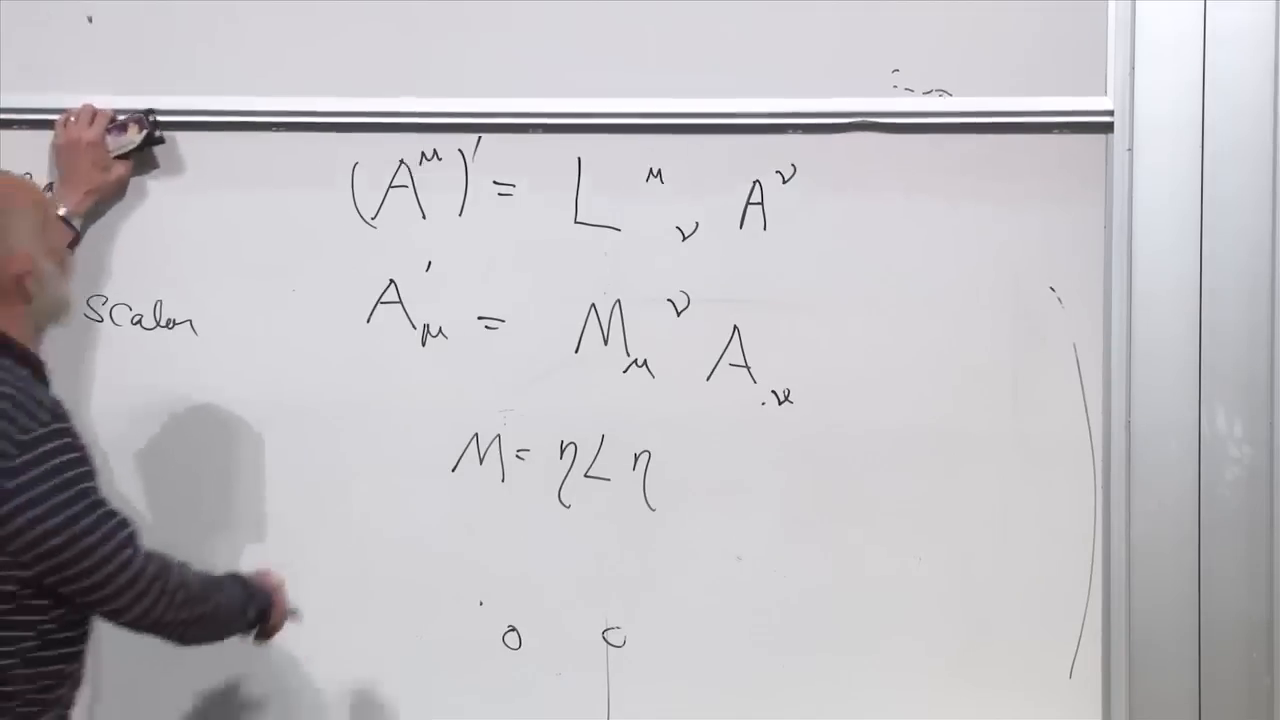
\includegraphics[width=0.90\textwidth]{lecture_06_figure_06.png}
\caption{逆变与协变变换律，二者由\(M=\eta L\eta\)相联系。}
\lectureframe{00:25:20}
\end{figure}

核心思想现在可以给出了：四维矢量是这样一种对象，其分量与时空坐标同步变换。

\section{张量：每个指标对应一个变换}

\subsection{从矢量乘积到定义}

标量是零阶张量，矢量是一阶张量，而带有两个指标的对象是二阶张量。从两个矢量出发，构造
\begin{equation}
T^{\mu\nu}=A^\mu B^\nu.
\label{eq:sr6-simple-tensor}
\end{equation}
共有\(4\times4=16\)个分量。它们从\(A^0B^0\)和
\(A^0B^1\)一直到\(A^3B^3\)。
符号\(T^{\mu\nu}\)表示整个这个阵列，而不是某一个数。

分别变换每个矢量，得到
\begin{align}
(A^\mu)'&=L^\mu{}_\sigma A^\sigma,\\
(B^\nu)'&=L^\nu{}_\tau B^\tau,
\end{align}
因此
\begin{equation}
(T^{\mu\nu})'
=
L^\mu{}_\sigma L^\nu{}_\tau T^{\sigma\tau}.
\label{eq:sr6-rank-two-transform}
\end{equation}
张量的每个指标都得到自己的洛伦兹矩阵。哑指标
\(\sigma\)和\(\tau\)可以随意改名，只要每一对保持前后一致即可。

\begin{classroomqa}
\audiencequestion{这种重新排列是否假定了矩阵与矢量分量可以对易？}
\lecturerresponse{它们是普通的经典数，而不是不可对易的量子算符，因此可以对易。此外，同一个洛伦兹矩阵同时作用于两个指标。这个计算中不存在次序问题。\lecturetimestamp{00:31:56}}
\end{classroomqa}

这条规则立即推广到三阶：
\begin{equation}
(T^{\mu\nu\lambda})'
=
L^\mu{}_\sigma
L^\nu{}_\tau
L^\lambda{}_\kappa
T^{\sigma\tau\kappa},
\label{eq:sr6-rank-three-transform}
\end{equation}
并同样推广到任意阶。正是这条变换律，而不是某种分解为矢量的特定方式，才是张量的定义。例如，
\begin{equation}
A^\mu B^\nu+C^\mu D^\nu
\end{equation}
仍然是张量，尽管它一般不能写成两个矢量的一个乘积。

\begin{figure}[htbp]
\centering
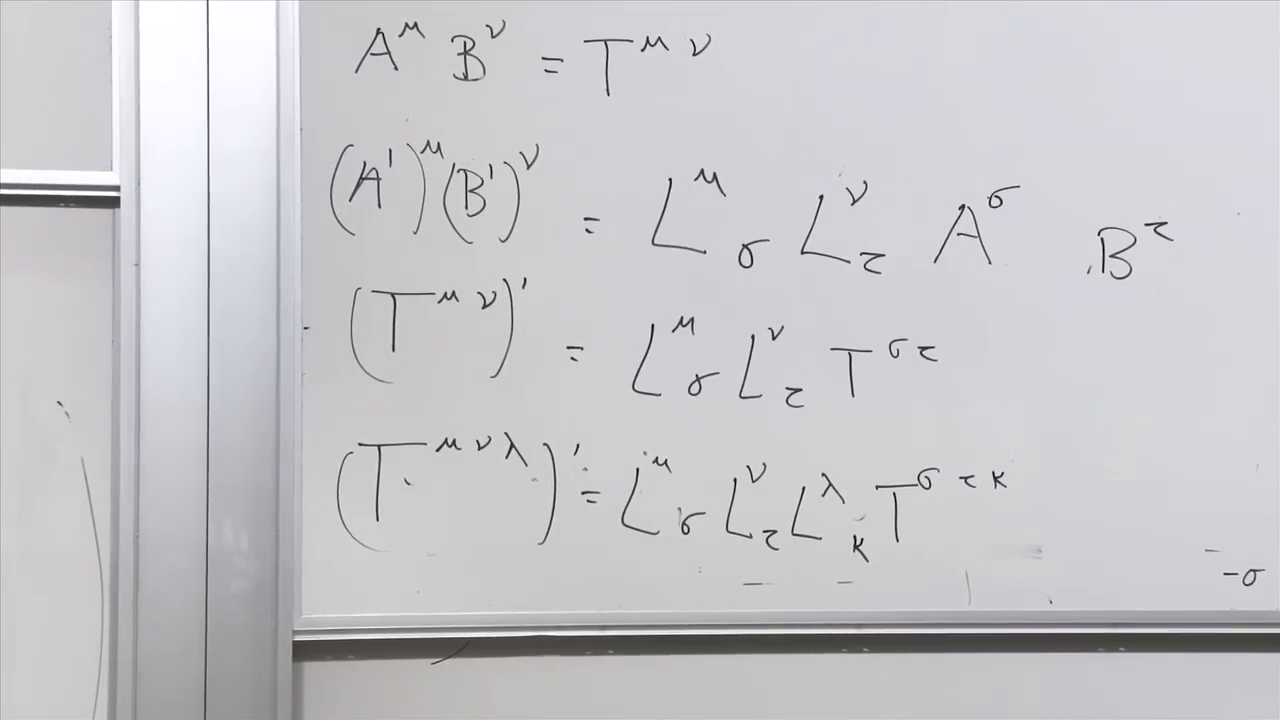
\includegraphics[width=0.90\textwidth]{lecture_06_figure_07.png}
\caption{从矢量乘积到二阶与三阶张量变换律的黑板推导阶梯。}
\lectureframe{00:33:20}
\end{figure}

\begin{classroomqa}
\audiencequestion{用一个二阶张量做矩阵乘法，逐分量来看是什么意思？}
\lecturerresponse{固定两个输出指标，对两个隐藏指标求和。例如，
\[
(T^{31})'=L^3{}_\sigma L^1{}_\tau T^{\sigma\tau}.
\]
由于\(\sigma\)和\(\tau\)都取四个值，这一个输出分量包含十六项。\lecturetimestamp{00:34:35}}
\end{classroomqa}

\begin{figure}[htbp]
\centering
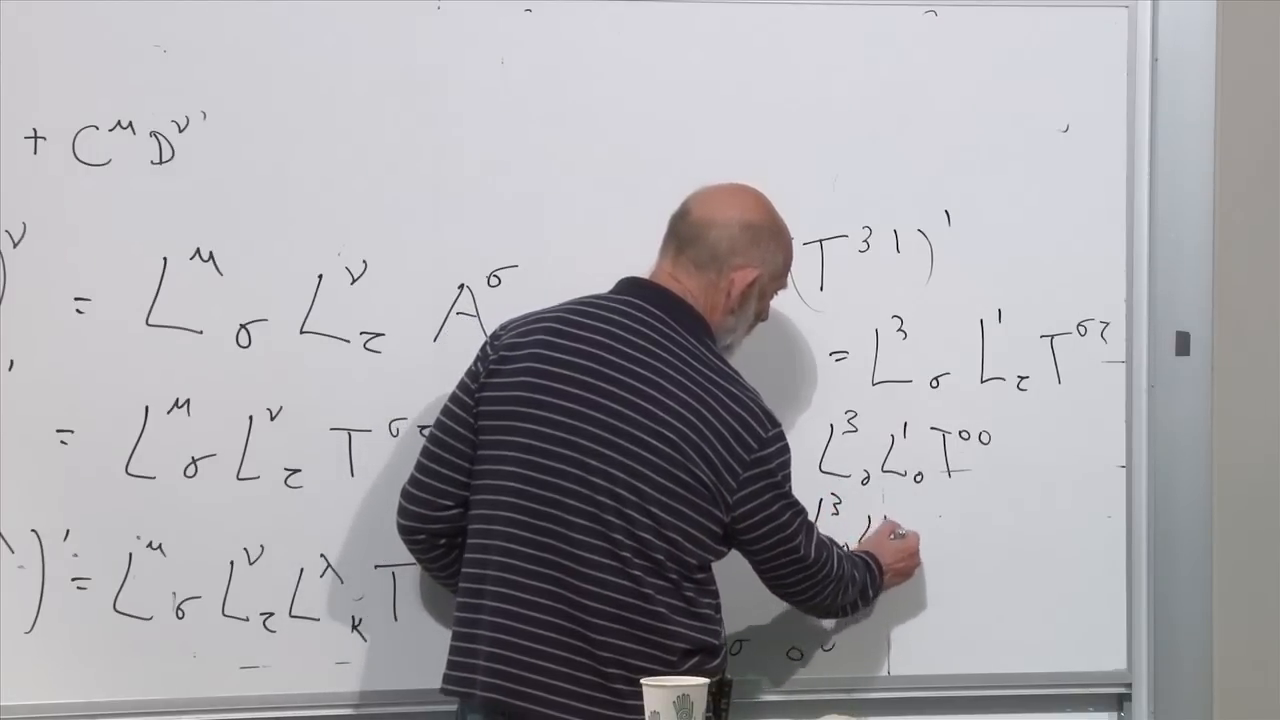
\includegraphics[width=0.90\textwidth]{lecture_06_figure_08.png}
\caption{展开固定的分量\((T^{31})'\)，使两个独立的求和变得显式。}
\lectureframe{00:35:55}
\end{figure}

张量方程具有决定性的优势。如果两个张量在某个参考系中分量相等，那么变换律使它们在每个参考系中都相等。等价地说，如果张量的每个分量在某个参考系中都为零，那么整个张量在每个参考系中都为零。仅有一个分量为零是不够的；所有分量都必须为零。这就是为什么写在张量之间的方程能将其真理性从一个惯性系传递到另一个惯性系。

\subsection{张量指标的升降}

张量的一个指标的下降方式与矢量的指标完全相同：
\begin{equation}
T^\mu{}_\nu=T^{\mu\sigma}\eta_{\sigma\nu}.
\label{eq:sr6-tensor-lowering}
\end{equation}
对于\eqref{eq:sr6-metric-lowering}中的对角度规，每下降一个时间指标就贡献一个负号。因此，
\begin{equation}
T_{00}=T^{00},
\qquad
T_{01}=-T^{01}.
\label{eq:sr6-tensor-component-signs}
\end{equation}
第一个等式中包含两次符号变化；第二个等式中只包含一次。

\begin{figure}[htbp]
\centering
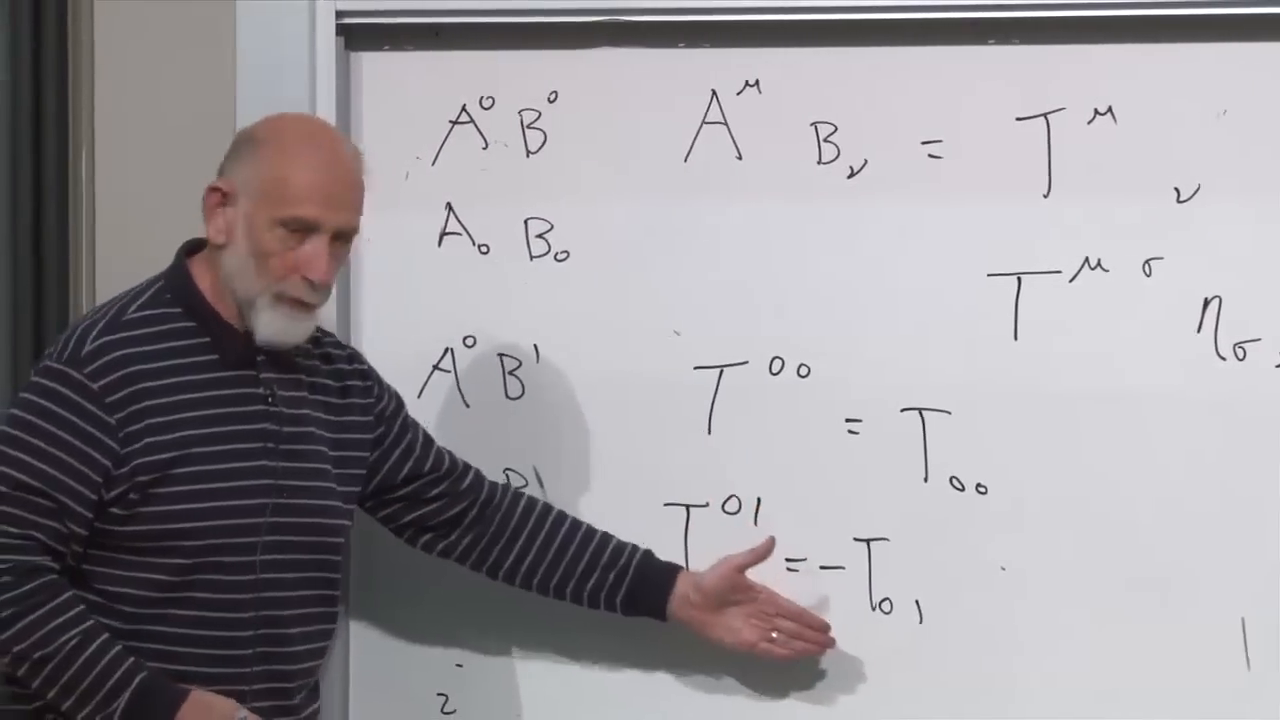
\includegraphics[width=0.90\textwidth]{lecture_06_figure_09.png}
\caption{下降两个张量指标的例子：两个时间指标给出两个负号，而一个时间指标给出一个负号。}
\lectureframe{00:41:00}
\end{figure}

\begin{classroomqa}
\audiencequestion{为什么同时保留协变形式和逆变形式是有用的？除了记号紧凑之外，还有更多意义吗？}
\lecturerresponse{就目前的计算而言，直接的好处是缩并紧凑，并能自动处理闵可夫斯基符号。矢量与余矢量之间还有更深的几何区别，但那更适合在广义相对论中展开。在平直时空中，指标规则如此高效，以至于人们通常直接使用它们。\lecturetimestamp{00:41:26}}
\end{classroomqa}

\begin{classroomqa}
\audiencequestion{张量总是有四个分量吗，还是说这是相对论特有的？}
\lecturerresponse{每个指标的取值范围由空间的维数决定。四维时空中的一阶张量有四个分量；二阶张量有十六个。在三维中，相应的数目是三和九。张量法则本身与维数无关。\lecturetimestamp{00:42:55}}
\end{classroomqa}

\begin{classroomqa}
\audiencequestion{协变对象和逆变对象能否用更几何的方式来描述？}
\lecturerresponse{可以，它们有几何解释，但现在深究会把电动力学推得更远。对本课程而言，变换规则和指标操作规则已经足够；几何上的区别在广义相对论中将变得不可回避。\lecturetimestamp{00:43:51}}
\end{classroomqa}

\section{对称性、反对称性与电磁张量}

对于一般的二阶张量，交换指标会改变分量：
\begin{equation}
T^{\mu\nu}\neq T^{\nu\mu}.
\end{equation}
确实，\(A^\mu B^\nu\) 与 \(A^\nu B^\mu\) 一般并不相同；具体分量 \(A^0B^1\) 与 \(A^1B^0\) 也不必相等。

有两个重要的特例。对称张量满足
\begin{equation}
T^{\mu\nu}=T^{\nu\mu},
\end{equation}
一个具体的对称组合是
\begin{equation}
A^\mu B^\nu+A^\nu B^\mu.
\end{equation}
反对称张量满足
\begin{equation}
F^{\mu\nu}=-F^{\nu\mu},
\label{eq:sr6-antisymmetry}
\end{equation}
组合
\begin{equation}
A^\mu B^\nu-A^\nu B^\mu.
\end{equation}
也是如此。在 \eqref{eq:sr6-antisymmetry} 中令两个指标相等，得到
\begin{equation}
F^{00}=-F^{00},
\qquad
F^{00}=0,
\end{equation}
同样的论证消去每一个对角分量。因此一个 \(4\times4\) 反对称张量有六个独立分量。

\begin{figure}[htbp]
\centering
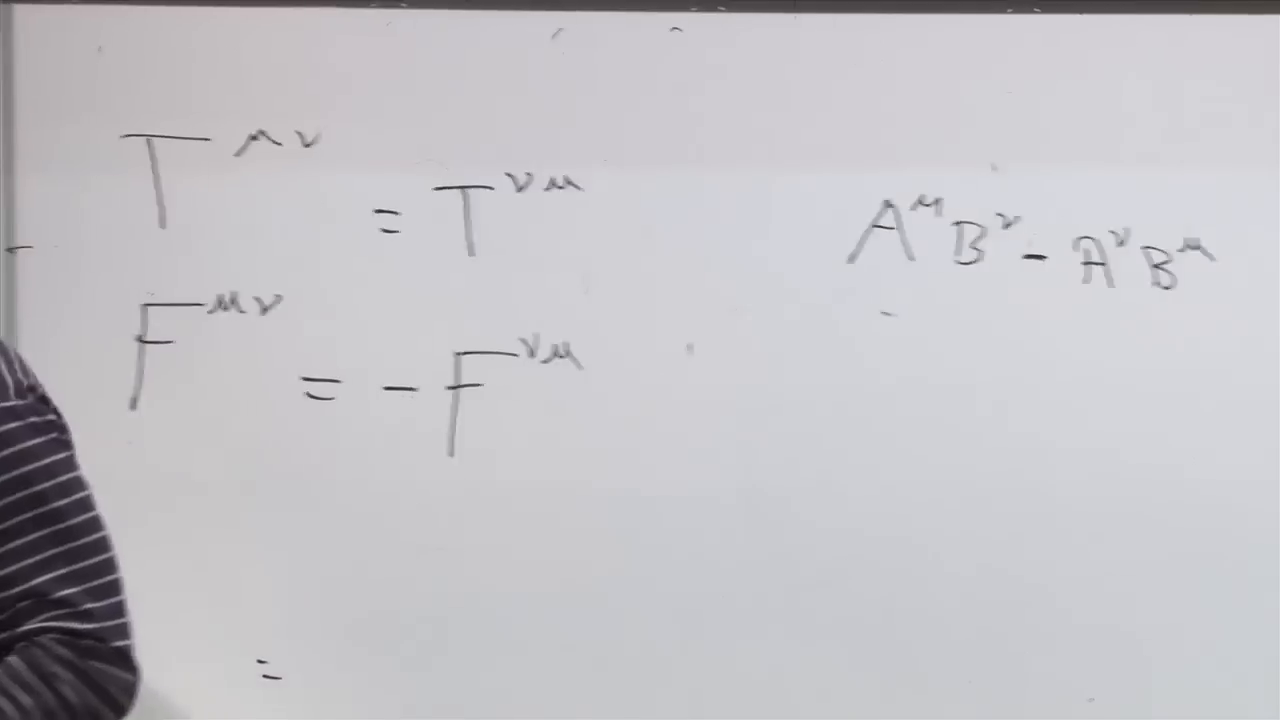
\includegraphics[width=0.90\textwidth]{lecture_06_figure_10.png}
\caption{在黑板上比较对称与反对称的二阶张量。}
\lectureframe{00:47:20}
\end{figure}

这六个分量恰好足以容纳电场的三个分量和磁场的三个分量。按照黑板上写下的符号约定，
\begin{equation}
F^{\mu\nu}
=
\begin{pmatrix}
0&-E_1&-E_2&-E_3\\
E_1&0&-B_3&B_2\\
E_2&B_3&0&-B_1\\
E_3&-B_2&B_1&0
\end{pmatrix}.
\label{eq:sr6-em-field-tensor}
\end{equation}
沿对角线反射会使每个符号反转。因此电场和磁场并不是彼此独立的相对论对象。一个助推可以像混合空间与时间那样混合它们：在一个参考系中纯电性的场，在另一个参考系中可能具有磁分量。

\begin{figure}[htbp]
\centering
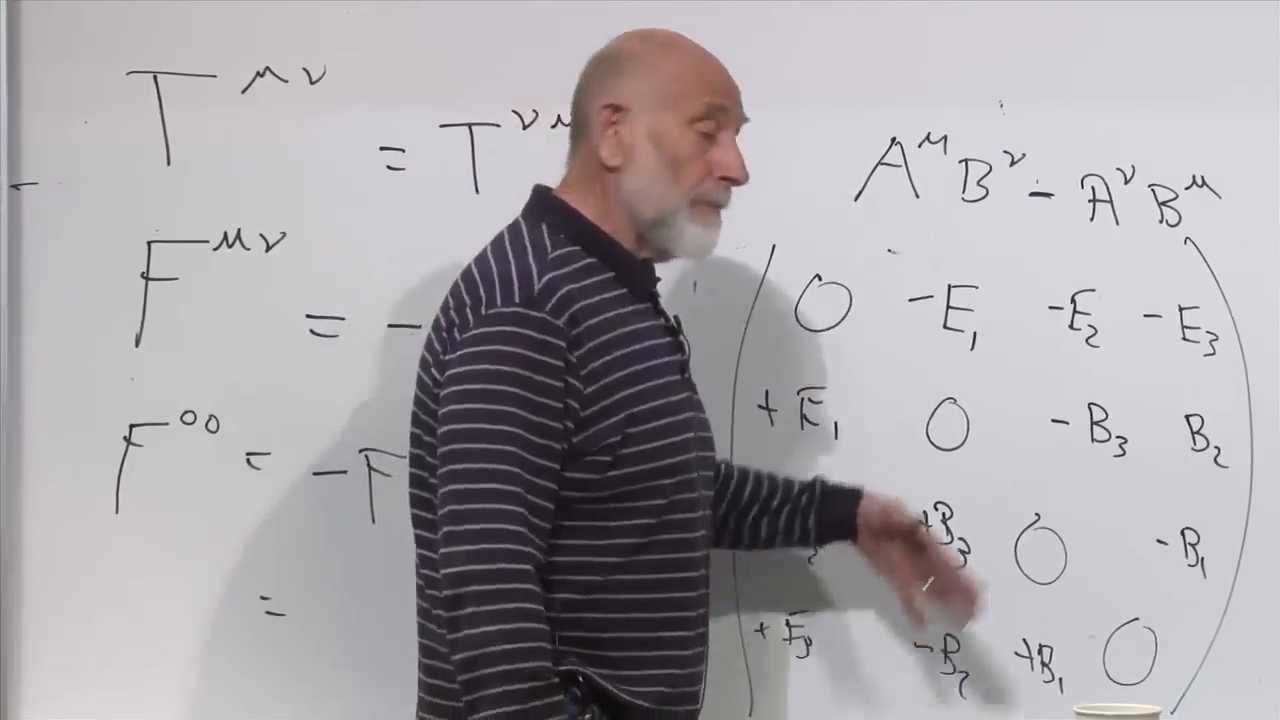
\includegraphics[width=0.90\textwidth]{lecture_06_figure_11.png}
\caption{完整的反对称阵列，其六个独立元素为 \(\mathbf E\) 和 \(\mathbf B\)。}
\lectureframe{00:50:20}
\end{figure}

写有 \eqref{eq:sr6-em-field-tensor} 的黑板仍然可见，讨论转向粒子动力学。现在我们重新使用符号 \(A_\mu\)，不是指前面例子中的一般矢量，而是指电磁四维势。

\section{带电粒子的作用量}

有两个可能的出发点。我们可以研究场本身的动力学，这将导向麦克斯韦方程；或者研究在给定场中运动的带电粒子，这将导向洛伦兹力。我们从粒子开始。

在低速下，目标是
\begin{equation}
m\mathbf a
=
e\left(\mathbf E+\mathbf v\times\mathbf B\right),
\label{eq:sr6-nonrel-lorentz-force}
\end{equation}
其中在采用高斯单位制的版本中，磁力项前有一个因子 \(1/c\)。我们令 \(c=1\)。在 \eqref{eq:sr6-nonrel-lorentz-force} 中的两项用三维矢量记号看起来不同，但相对论应当揭示它们是同一个对象的组成部分。

\begin{figure}[htbp]
\centering
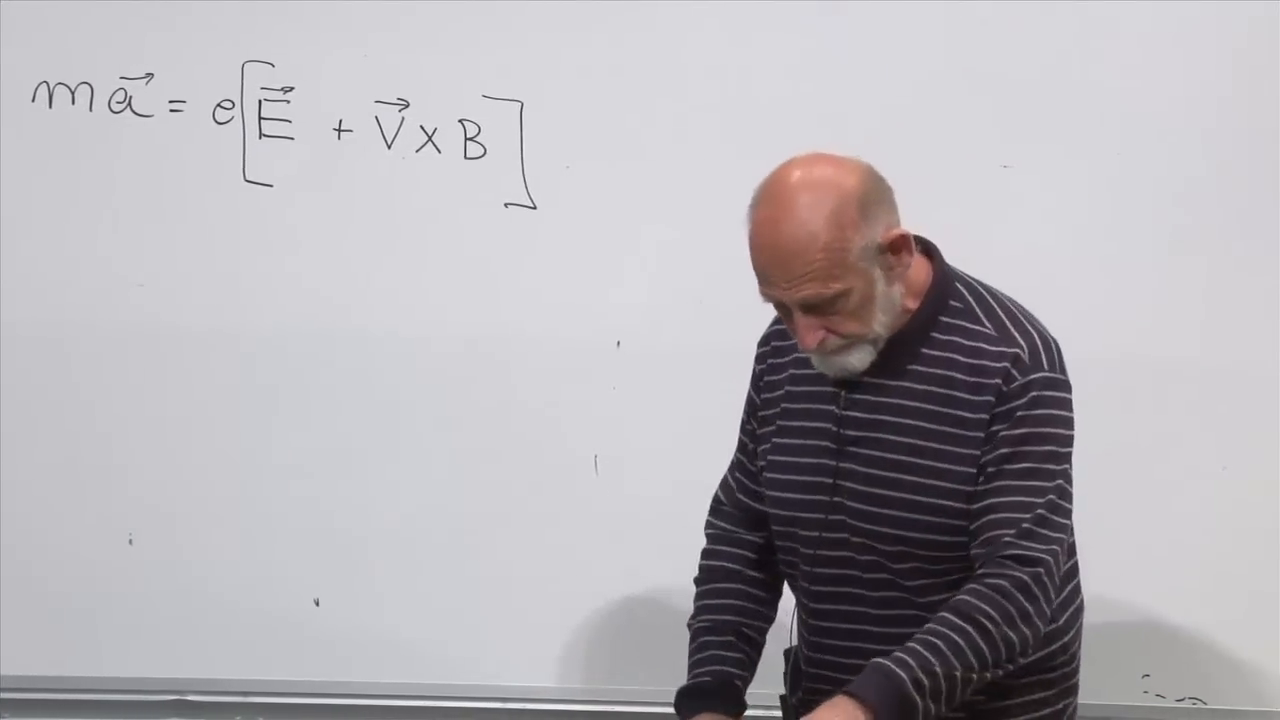
\includegraphics[width=0.90\textwidth]{lecture_06_figure_12.png}
\caption{非相对论洛伦兹力，即不变作用量必须重现的结果。}
\lectureframe{00:54:00}
\end{figure}

\subsection{自由运动与矢量势}

对于自由相对论粒子，
\begin{equation}
S_{\mathrm{free}}
=
-m\int_1^2 d\tau
=
\int_{t_1}^{t_2}dt\,
\left[-m\sqrt{1-\dot{\mathbf x}^{\,2}}\right],
\label{eq:sr6-free-action}
\end{equation}
其中
\begin{equation}
\dot{\mathbf x}^{\,2}
=
(\dot x^1)^2+(\dot x^2)^2+(\dot x^3)^2.
\end{equation}
方括号中的量就是自由粒子拉格朗日量。它的动量和能量此前已经求出；我们保留作用量，并追问可以加入什么样的依赖于场的项。

\begin{figure}[htbp]
\centering
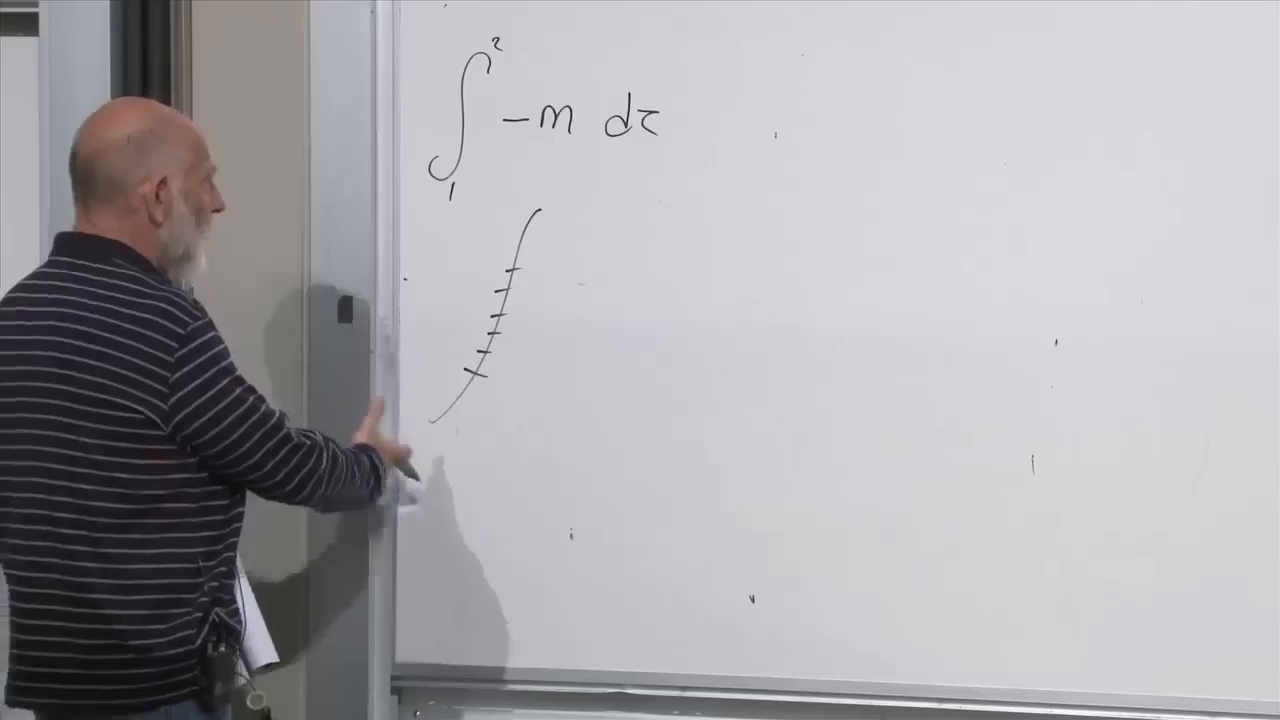
\includegraphics[width=0.90\textwidth]{lecture_06_figure_13.png}
\caption{自由作用量作为沿世界线累积的固有时。}
\lectureframe{00:55:10}
\end{figure}

基本的电磁变量是四维矢量势
\(A_\mu(x)\)。电场和磁场将由它导出。沿一小段世界线 \(dx^\mu\)，缩并
\begin{equation}
A_\mu(x)\,dx^\mu
\end{equation}
是一个标量。把这些标量增量从一个端点到另一个端点相加，就给出一个洛伦兹不变的相互作用：
\begin{equation}
S_{\mathrm{int}}
=
-e\int_1^2 A_\mu(x)\,dx^\mu.
\label{eq:sr6-interaction-action}
\end{equation}
系数 \(e\) 是电荷。整体的符号属于历史上的电荷约定；改变约定只会改变赋予 \(e\) 的符号，而不会改变理论的内容。

\begin{figure}[htbp]
\centering
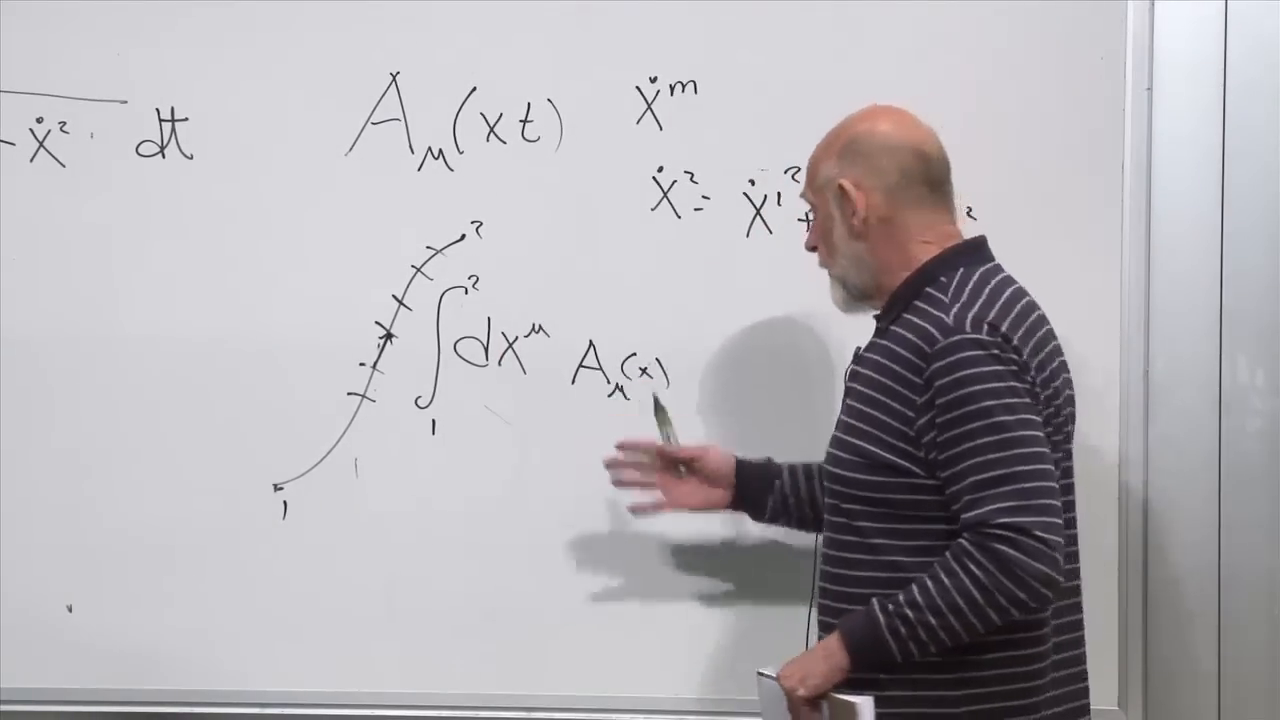
\includegraphics[width=0.90\textwidth]{lecture_06_figure_14.png}
\caption{一段世界线与四维势缩并，构成标量增量 \(A_\mu dx^\mu\)。}
\lectureframe{00:59:20}
\end{figure}

\subsection{普通时间形式}

为了使用熟悉的欧拉--拉格朗日方程，把 \eqref{eq:sr6-interaction-action} 除以并乘以 \(dt\)。由于
\begin{equation}
\frac{dx^0}{dt}=1,
\qquad
\frac{dx^m}{dt}=\dot x^m,
\end{equation}
完整的作用量为
\begin{equation}
S
=
\int dt\,
\left[
-m\sqrt{1-\dot{\mathbf x}^{\,2}}
-eA_0(x,t)
-e\dot x^m A_m(x,t)
\right].
\label{eq:sr6-complete-particle-action}
\end{equation}
因此
\begin{equation}
\boxed{
L
=
-m\sqrt{1-\dot{\mathbf x}^{\,2}}
-eA_0
-e\dot x^mA_m
}.
\label{eq:sr6-charged-lagrangian}
\end{equation}
目前 \(A_\mu(x,t)\) 是已知的外场。我们变分世界线，而不是变分场。

\begin{figure}[htbp]
\centering
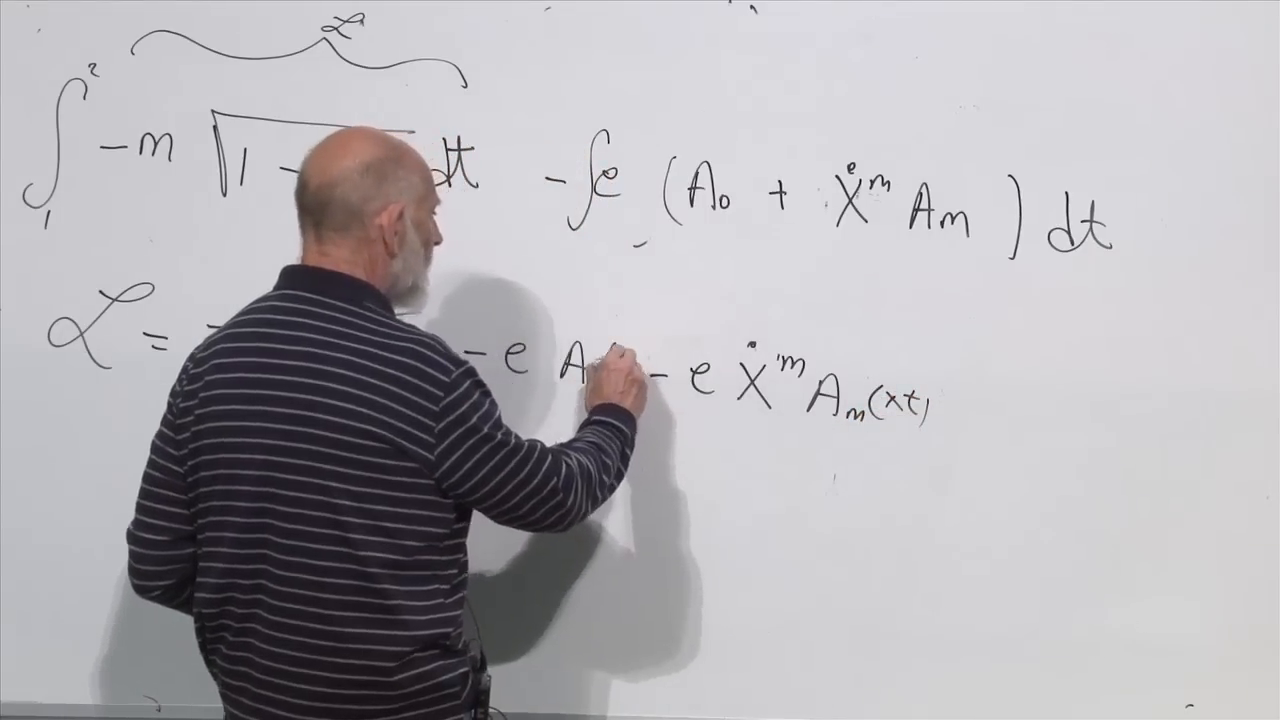
\includegraphics[width=0.90\textwidth]{lecture_06_figure_15.png}
\caption{将不变世界线耦合改写为普通时间下的拉格朗日量。}
\lectureframe{01:05:20}
\end{figure}

\section{推导洛伦兹力}

对于空间分量 \(x^m\)，欧拉--拉格朗日方程为
\begin{equation}
\frac{d}{dt}\frac{\partial L}{\partial\dot x^m}
=
\frac{\partial L}{\partial x^m}.
\label{eq:sr6-EL}
\end{equation}
对速度求导得到
\begin{equation}
\frac{\partial L}{\partial\dot x^m}
=
\frac{m\dot x_m}{\sqrt{1-\dot{\mathbf x}^{\,2}}}
-eA_m.
\label{eq:sr6-canonical-momentum}
\end{equation}
字母 \(m\) 不幸既表示质量又表示空间指标。上下文可以区分它们：\eqref{eq:sr6-canonical-momentum} 中的第一个 \(m\) 是质量；下标 \(m\) 标记三个空间分量之一。

\begin{figure}[htbp]
\centering
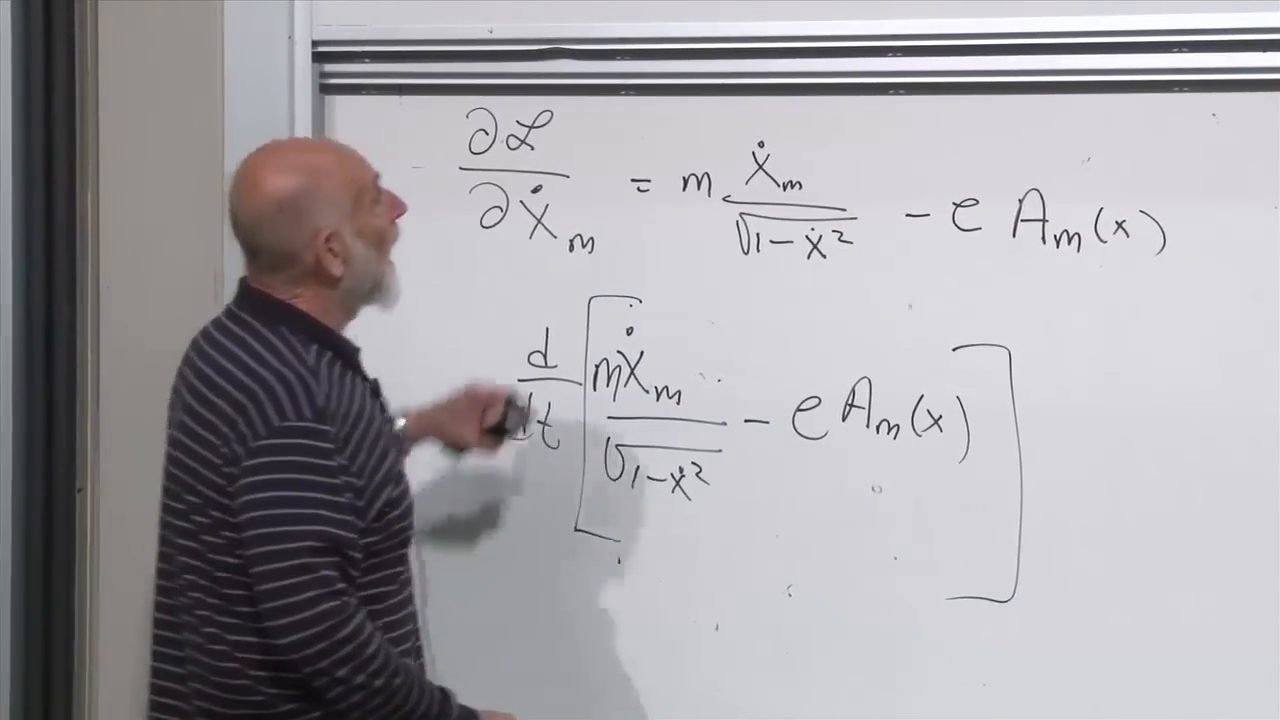
\includegraphics[width=0.90\textwidth]{lecture_06_figure_16.png}
\caption{动量导数既包含力学项，也包含矢量势项。}
\lectureframe{01:09:20}
\end{figure}

\begin{classroomqa}
\audiencequestion{左边第一次尝试是否漏掉了一项？}
\lecturerresponse{是的。只对自由粒子项求导会遗漏 \(-e\dot x^mA_m\) 对速度的依赖。完整的导数是 \(m\dot x_m/\sqrt{1-\dot{\mathbf x}^{\,2}}-eA_m\)。这一修正至关重要，因为它的时间导数同时提供了电场力和磁场力的一部分。\lecturetimestamp{01:08:18}}
\end{classroomqa}

\eqref{eq:sr6-EL} 的右边是
\begin{equation}
\frac{\partial L}{\partial x^m}
=
-e\,\partial_mA_0
-e\,\dot x^n\partial_mA_n.
\label{eq:sr6-position-derivative}
\end{equation}
因此
\begin{equation}
\frac{d}{dt}
\left(
\frac{m\dot x_m}{\sqrt{1-\dot{\mathbf x}^{\,2}}}
-eA_m
\right)
=
-e\,\partial_mA_0
-e\,\dot x^n\partial_mA_n.
\label{eq:sr6-EL-expanded}
\end{equation}

\begin{classroomqa}
\audiencequestion{在这个计算中，协变和逆变空间分量是否被互换了？}
\lecturerresponse{它们被升降了，但对于拉丁空间指标，度规的欧几里得空间块是单位矩阵。因此 \(x_m=x^m\) 且 \(A_m=A^m\)。只有时间指标才会产生符号变化。\lecturetimestamp{01:09:29}}
\end{classroomqa}

\begin{classroomqa}
\audiencequestion{重复的拉丁指标也要求和吗？}
\lecturerresponse{是的。重复的拉丁指标从 \(1\) 求和到 \(3\)；重复的希腊指标从 \(0\) 求和到 \(3\)。像 \(m\) 这样标记一个空间方程的单独指标是自由指标，不求和。质量符号不是指标。\lecturetimestamp{01:10:00}}
\end{classroomqa}

\begin{figure}[htbp]
\centering
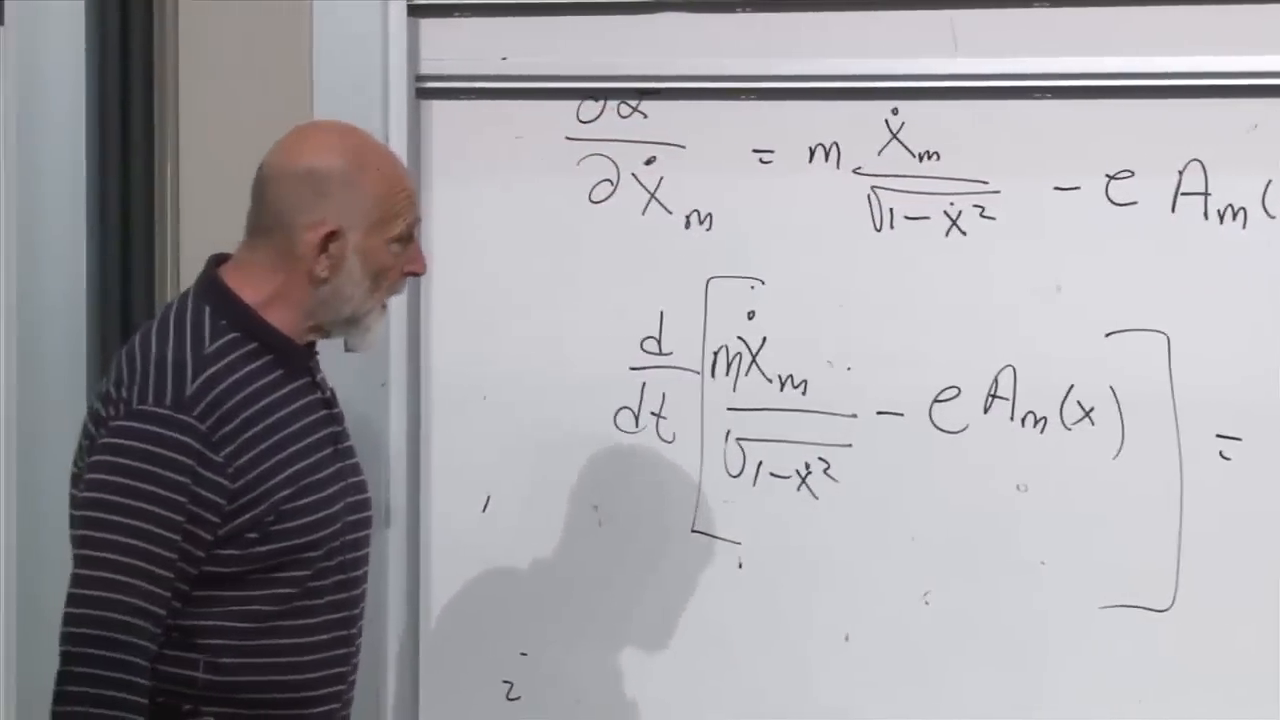
\includegraphics[width=0.90\textwidth]{lecture_06_figure_17.png}
\caption{在展开矢量势的全时间导数之前的欧拉--拉格朗日方程。}
\lectureframe{01:14:20}
\end{figure}

\subsection{沿运动世界线的链式法则}

即使场不随时间变化，它也会沿粒子路径变化，因为粒子采样了不同的位置。全导数为
\begin{equation}
\frac{dA_m(x(t),t)}{dt}
=
\partial_0A_m+\dot x^n\partial_nA_m.
\label{eq:sr6-convective-derivative}
\end{equation}
第一项是显式时间依赖；第二项是通过 \(x^n(t)\) 的隐式时间依赖。

\begin{figure}[htbp]
\centering
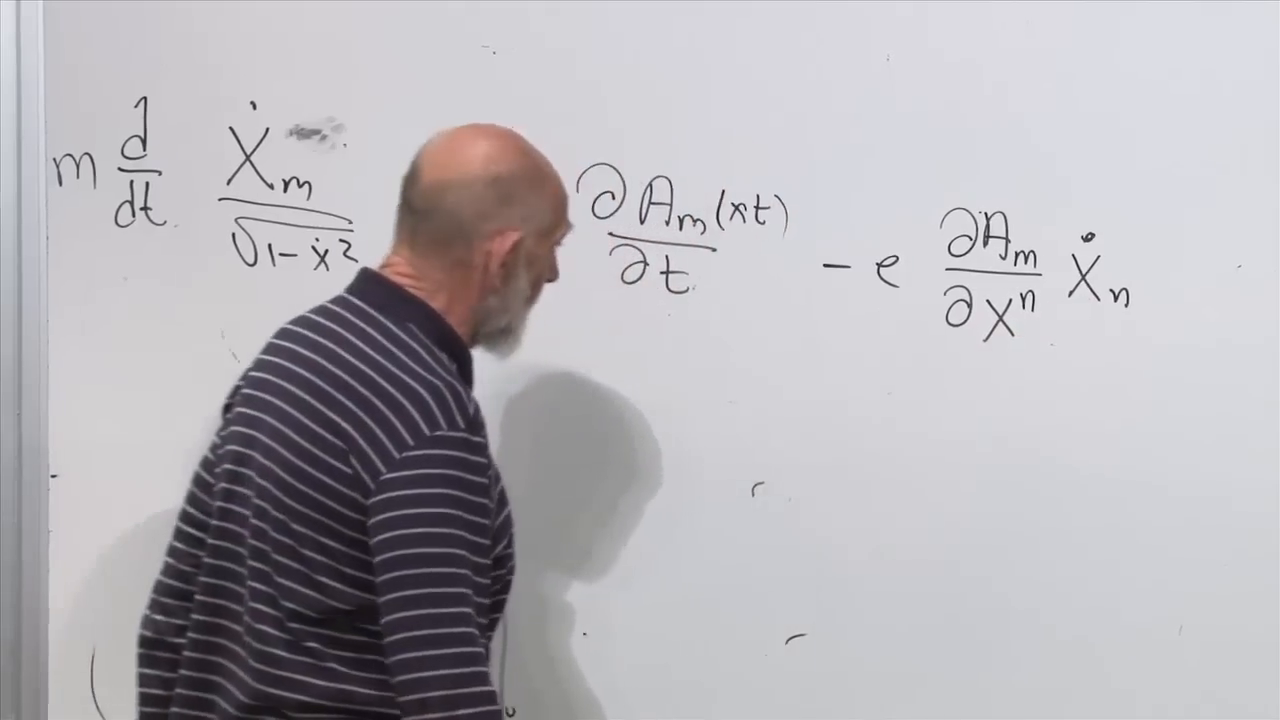
\includegraphics[width=0.90\textwidth]{lecture_06_figure_18.png}
\caption{矢量势随时间显式变化，并随粒子在空间中运动而隐式变化。}
\lectureframe{01:17:20}
\end{figure}

将 \eqref{eq:sr6-convective-derivative} 代入
\eqref{eq:sr6-EL-expanded} 并把场项移到右边，得到
\begin{equation}
\begin{aligned}
m\frac{d}{dt}
\left(
\frac{\dot x_m}{\sqrt{1-\dot{\mathbf x}^{\,2}}}
\right)
&=
e\left(\partial_0A_m-\partial_mA_0\right)
\\
&\quad +e\dot x^n
\left(\partial_nA_m-\partial_mA_n\right).
\end{aligned}
\label{eq:sr6-grouped-force}
\end{equation}
这个计算终于找到了它的组织原则。第一个括号不含速度；第二个对速度是线性的。这正是电场力与磁场力之间的划分。

\begin{figure}[htbp]
\centering
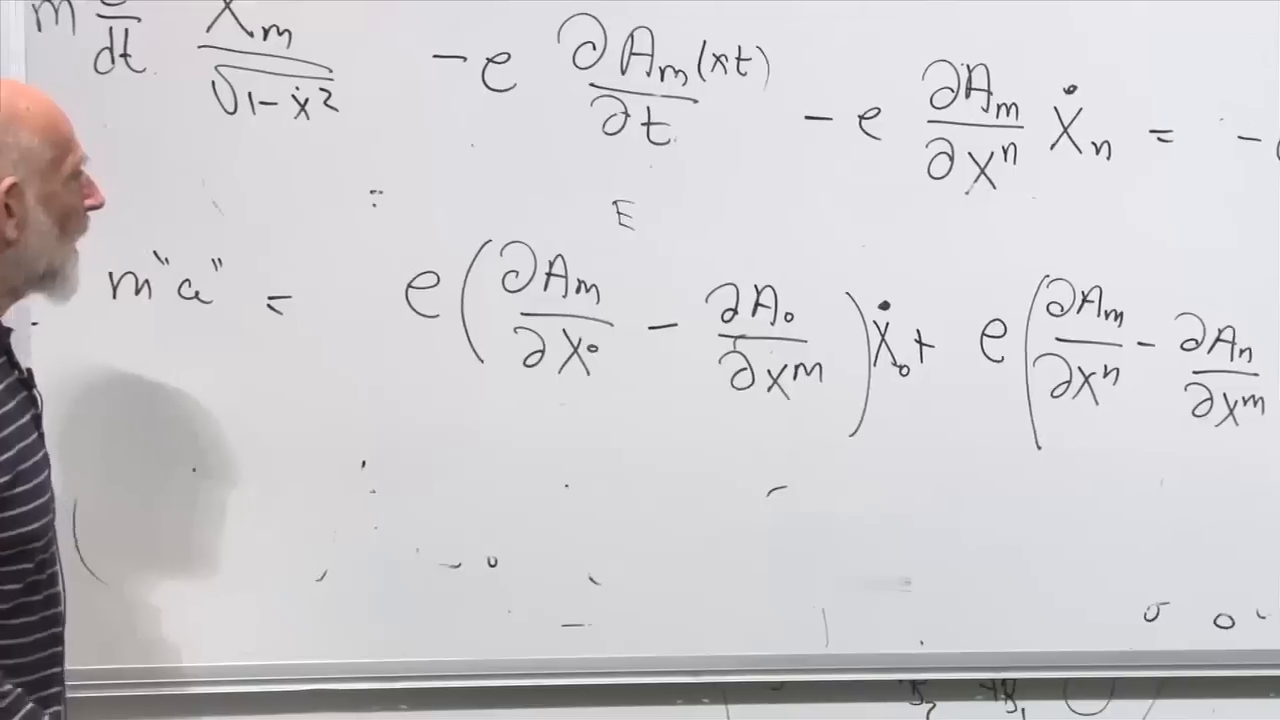
\includegraphics[width=0.90\textwidth]{lecture_06_figure_19.png}
\caption{力项被归并为与速度无关的电场部分和与速度相关的反对称部分。}
\lectureframe{01:23:40}
\end{figure}

按照推导中的约定，定义电场分量为
\begin{equation}
E_m=\partial_0A_m-\partial_mA_0.
\label{eq:sr6-electric-from-potential}
\end{equation}
空间反对称组合
\begin{equation}
C_{mn}
\equiv
\partial_nA_m-\partial_mA_n
\label{eq:sr6-spatial-curl-tensor}
\end{equation}
包含矢量势旋度的三个独立分量。其取向选择得使
\begin{equation}
\dot x^nC_{mn}
=
\left(\mathbf v\times\mathbf B\right)_m.
\end{equation}
因此，方程 \eqref{eq:sr6-grouped-force} 是 \eqref{eq:sr6-nonrel-lorentz-force} 的相对论动量形式。时间导数下的因子是单位质量的相对论动量，而不只是牛顿速度。

这个推导值得亲手重复一遍：从
\eqref{eq:sr6-charged-lagrangian} 出发，计算
\eqref{eq:sr6-EL} 的两边，应用链式法则，并按速度依赖性归并各项。这个练习同时是变分力学、多变量微积分和电动力学的训练。

\begin{classroomqa}
\audiencequestion{为什么选择 \(-e\int A_\mu dx^\mu\) 作为电磁相互作用？}
\lecturerresponse{最终由实验决定耦合，但两个结构性要求使这成为自然的第一个候选。作用量由沿轨迹的局域增量组装而成，而每个增量都必须是标量。标量 \(dx^\mu dx_\mu=d\tau^2\) 已经由自由作用量表示。将 \(dx^\mu\) 与场 \(A_\mu\) 缩并是最简单的新的依赖场的标量。可以写出更复杂的标量，而规范不变性稍后会进一步收紧这一选择。\lecturetimestamp{01:25:34}}
\end{classroomqa}

\begin{classroomqa}
\audiencequestion{麦克斯韦方程组也能从最小作用量原理推导出来吗？}
\lecturerresponse{能。当前的作用量描述给定电磁场中的粒子。要得到麦克斯韦方程组，我们必须加上场自身的作用量，并对场本身变分，正如我们对标量场所做的那样。\lecturetimestamp{01:28:58}}
\end{classroomqa}

\begin{classroomqa}
\audiencequestion{分组后的力方程中的求和在哪里？}
\lecturerresponse{自由指标\(m\)标记三个分量方程之一，并不求和。\(\dot x^n(\partial_nA_m-\partial_mA_n)\)中重复的\(n\)对\(1,2,3\)求和。若不用爱因斯坦记号写出，该项会带有一个显式的\(\sum_{n=1}^{3}\)。\lecturetimestamp{01:29:26}}
\end{classroomqa}

\begin{classroomqa}
\audiencequestion{为什么把\(\partial_0A_m-\partial_mA_0\)认定为电场，而不是预先假设通常的公式？}
\lecturerresponse{作用量产生了一个力项，它依赖于位置和时间，但不依赖于粒子速度。这正是电场的操作角色。其余反对称项乘以速度，因而具有磁的角色。可以把这一计算看作从力定律发现场，而不是事先插入各自独立的定义。\lecturetimestamp{01:31:05}}
\end{classroomqa}

\section{显式协变的力定律}

\eqref{eq:sr6-grouped-force}的左边尚未写成明显的四维形式。引入四维速度
\begin{equation}
u^\mu=\frac{dx^\mu}{d\tau}.
\label{eq:sr6-four-velocity}
\end{equation}
其空间分量满足
\begin{equation}
u^m
=
\frac{dx^m}{d\tau}
=
\frac{\dot x^m}{\sqrt{1-\dot{\mathbf x}^{\,2}}}.
\end{equation}
将空间方程乘以\(dt/d\tau\)把\(d/dt\)转换为\(d/d\tau\)：
\begin{equation}
\frac{dt}{d\tau}\frac{d}{dt}
=
\frac{d}{d\tau}.
\end{equation}
因此左边成为固有加速度的空间部分，
\begin{equation}
m\frac{d^2x^m}{d\tau^2}.
\end{equation}

右边可以不分离时间和空间地写出：
\begin{equation}
m\frac{d^2x^m}{d\tau^2}
=
e\left(\partial_\nu A_m-\partial_mA_\nu\right)
\frac{dx^\nu}{d\tau}.
\label{eq:sr6-spatial-covariant-force}
\end{equation}
对于\(\nu=0\)，这重现电的括号；对于\(\nu=1,2,3\)，它重现磁的括号。

两边现在都具有四维矢量的变换性质。因此三个空间方程是
\begin{equation}
\boxed{
m\frac{d^2x^\mu}{d\tau^2}
=
e\left(\partial_\nu A^\mu-\partial^\mu A_\nu\right)u^\nu
}.
\label{eq:sr6-covariant-force}
\end{equation}
的分量。若定义
\begin{equation}
F_{\mu\nu}
\equiv
\partial_\mu A_\nu-\partial_\nu A_\mu,
\label{eq:sr6-F-from-A}
\end{equation}
则本讲所用的指标顺序和相互作用符号给出等价的紧凑形式
\begin{equation}
m\frac{du^\mu}{d\tau}
=
-eF^\mu{}_\nu u^\nu.
\label{eq:sr6-covariant-force-F}
\end{equation}
\editorialnote{电动力学教材在度规号差、\(A_\mu\)的定义、电荷以及\(F_{\mu\nu}\)之间以不同方式分配符号。方程\eqref{eq:sr6-covariant-force}和\eqref{eq:sr6-covariant-force-F}保留由作用量\(-e\int A_\mu dx^\mu\)得到的符号和指标顺序；不变的内容是势的反对称化导数。}

\begin{figure}[htbp]
\centering
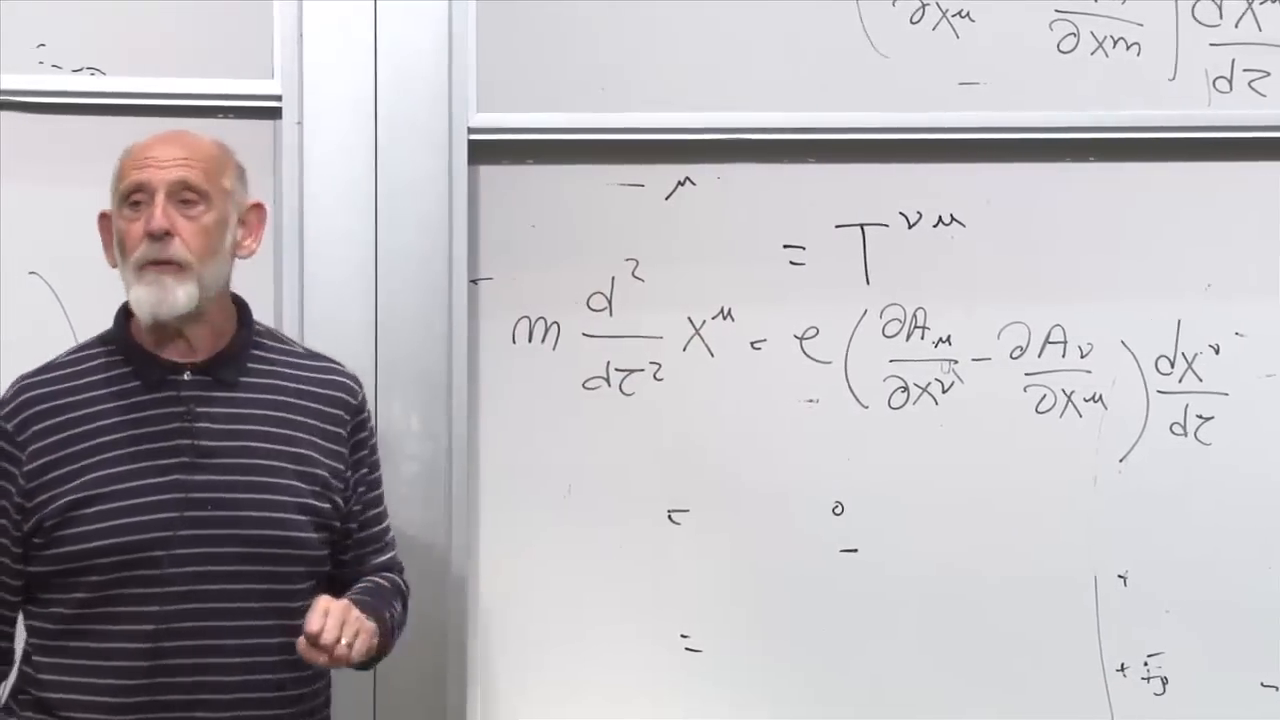
\includegraphics[width=0.90\textwidth]{lecture_06_figure_20.png}
\caption{用固有时间把三个空间方程组装成一个四维矢量方程。}
\lectureframe{01:42:40}
\end{figure}

\begin{classroomqa}
\audiencequestion{为什么可以合法地添加第四个时间分量方程？\(d^2x^0/d\tau^2\)是否简单地为零？}
\lecturerresponse{它一般不为零：\(x^0=t\)，但当粒子的速率变化时\(dt/d\tau=\gamma\)会改变。决定性的论据是协变性。标量作用量保证洛伦兹不变的方程；一旦空间分量被认定为一个四维矢量方程的分量，洛伦兹变换就会把它们与时间分量混合。第四个方程必须与其他三个相伴。\lecturetimestamp{01:42:40}}
\end{classroomqa}

\subsection{第四个分量的含义}

三个空间分量是相对论陈述
\begin{equation}
\frac{d\mathbf p}{dt}=\mathbf F.
\end{equation}
能量和动量本身是四维矢量的分量，所以时间分量必须描述相应的能量平衡。用三维矢量语言，
\begin{equation}
\frac{dK}{dt}=\mathbf F\cdot\mathbf v.
\label{eq:sr6-work-energy}
\end{equation}
它记录场对粒子做功的速率。磁的贡献垂直于\(\mathbf v\)，不做功；电的贡献改变粒子能量。

\begin{classroomqa}
\audiencequestion{如果协变性在形式上提供了第四个方程，我们怎么知道它具有物理意义？}
\lecturerresponse{前三个分量说力改变动量。第四个说功改变能量：\(dK/dt=\mathbf F\cdot\mathbf v\)。既然能量和动量构成一个四维矢量，它们对场的响应也必须是一个四分量的陈述。\lecturetimestamp{01:45:20}}
\end{classroomqa}

\begin{figure}[htbp]
\centering
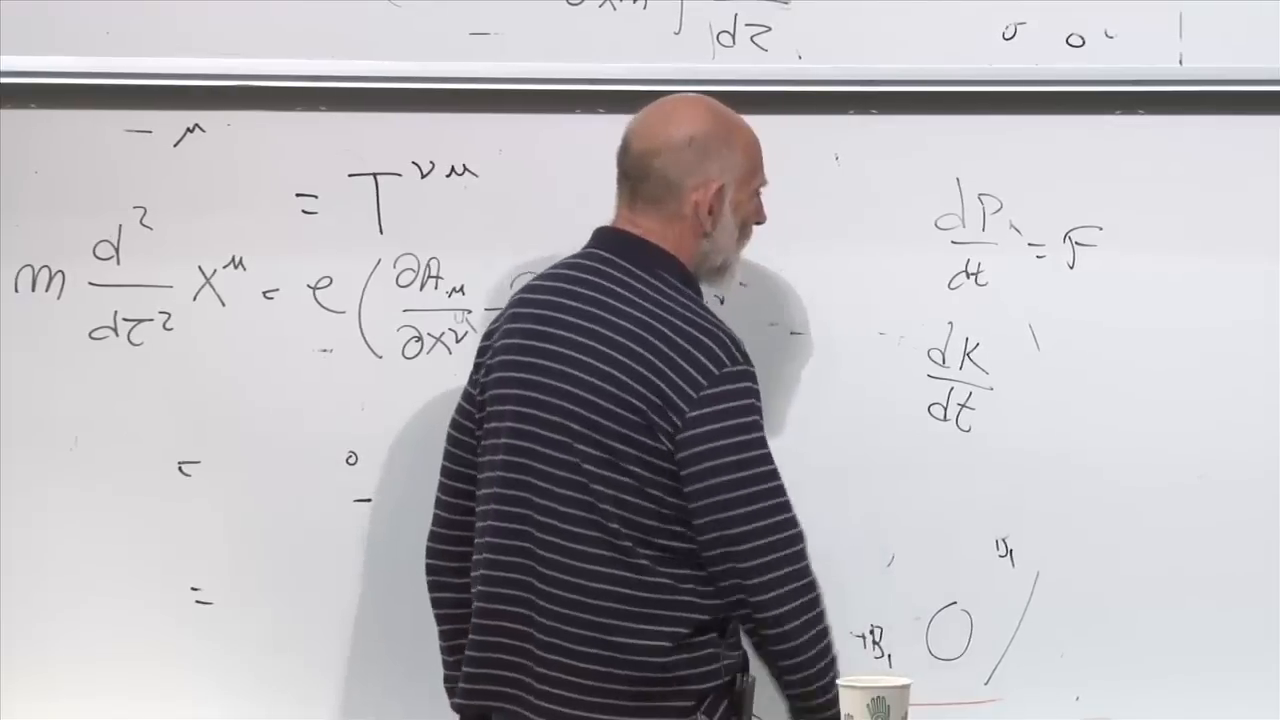
\includegraphics[width=0.90\textwidth]{lecture_06_figure_21.png}
\caption{空间定律\(d\mathbf p/dt=\mathbf F\)及其时间分量伙伴，即功--能关系。}
\lectureframe{01:47:10}
\end{figure}

方法比最终的压缩更重要。我们在变分之前要求作用量是标量。由此得到的方程随后可以被重新组织成张量，而不必事后修补其对称性。在现代场论中，这成为一条普遍的设计规则：构造拉格朗日量时要尊重问题的对称性。

\section{局域性、洛伦兹不变性与下一个对称性}

三个原理在相对论场论中反复出现。其中两个已经使用；第三个将在接下来展开。

\subsection{局域性}

定域性说的是，粒子或场的变化由时空中无穷邻近处发生的事所支配。粒子响应的是在其世界线上取值的场，而不是远处某个无关的取值。某一点处的场响应的是该点邻域内的场及其导数，而不是直接响应任意远处的取值或未来的数据。

因此，对于场，作用量取定域形式
\begin{equation}
S
=
\int d^3x\,dt\,
\mathcal L\!\left(\phi,\partial_\mu\phi\right).
\label{eq:sr6-local-action}
\end{equation}
该积分对每个时空点各贡献一项。一阶导数编码了与邻近点的比较，而变分原理则给出微分方程。人们可以设想把相距遥远的点处的场耦合起来的非定域乘积，但那样的方程会使此处的响应直接依赖于彼处的条件。那不是这里所要施加的定域结构。含高阶导数的作用量是可能的，并且构成一个有趣的课题，但目前的构造并不需要它们。

\begin{figure}[htbp]
\centering
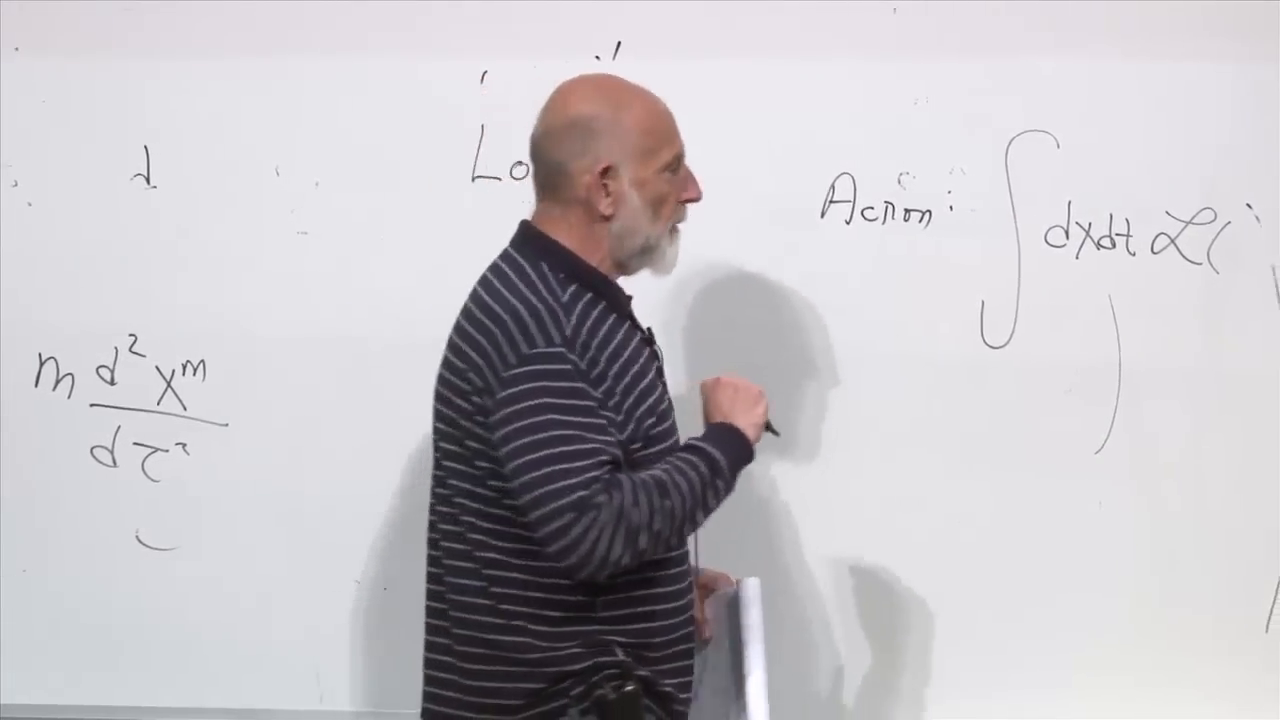
\includegraphics[width=0.90\textwidth]{lecture_06_figure_22.png}
\caption{定域性，表示为场及其邻近导数所构成的密度在时空上的积分。}
\lectureframe{01:51:00}
\end{figure}

\begin{classroomqa}
\audiencequestion{\(\partial_\mu\phi\)是否表示四个导数分量？}
\lecturerresponse{是的。它表示\(\phi\)的时间导数和三个空间导数，合为一个协变四维矢量。\lecturetimestamp{01:52:25}}
\end{classroomqa}

\begin{classroomqa}
\audiencequestion{在定域性原理中，\emph{邻近}是如何被量化的？}
\lecturerresponse{通过导数。一阶导数将某点处的场与其在无穷邻近点处的取值相比较。定域拉格朗日量依赖于场以及同一时空点处有限个这样的导数。\lecturetimestamp{01:52:55}}
\end{classroomqa}

\begin{classroomqa}
\audiencequestion{定域性的场论版本如何对应到刚刚完成的粒子计算？}
\lecturerresponse{粒子拉格朗日量沿世界线是定域的：它通过速度依赖于邻近的世界线位置，并依赖于在粒子当前位置处取值的电磁势。此处粒子的加速度并不直接依赖于远处某点处的场。\lecturetimestamp{01:53:31}}
\end{classroomqa}

\subsection{洛伦兹不变性}

洛伦兹不变性是通过用标量构造拉格朗日量来实现的。不同观测者可以把这些标量分解为不同的时间和空间分量，但他们对作用量的看法一致。因此，由变分得到的张量方程在每个惯性系中都具有相同的形式。

\subsection{规范不变性}

规范不变性是剩下的原理。这里只是宣告了它，尚未给出定义。在下一步中，它将限制四维势的哪些特征是物理上有意义的，并将引导出产生麦克斯韦方程组的场作用量。

\begin{figure}[htbp]
\centering
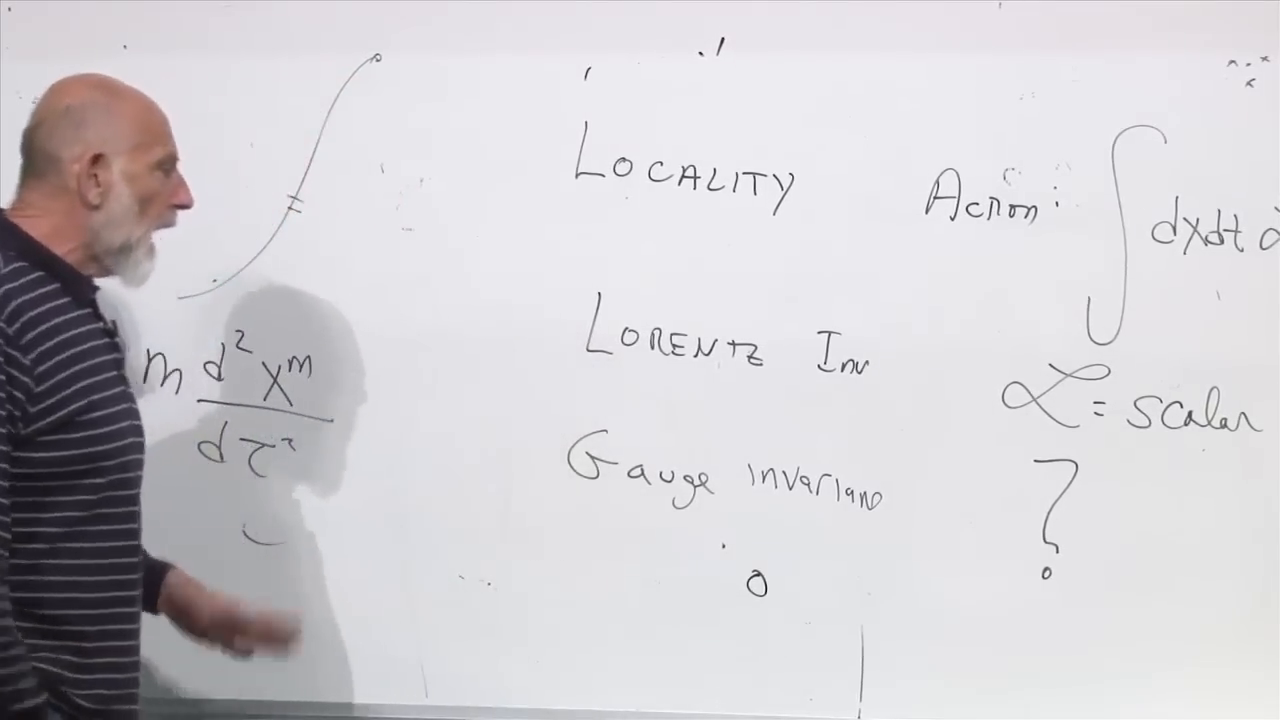
\includegraphics[width=0.90\textwidth]{lecture_06_figure_23.png}
\caption{三条组织性原理：定域性、洛伦兹不变性和规范不变性。}
\lectureframe{01:55:40}
\end{figure}

这些原理在广义相对论、量子电动力学、杨--米尔斯理论以及标准模型中反复出现。诸如粒子种类数目之类的细节因理论而异；定域性和对称性提供了更深刻的框架。因此，实际的作业是重新追溯欧拉--拉格朗日计算，直到每一个指标和每一个成组的项都能得到说明。随后，规范不变性将作为对同一电磁作用量的下一个约束而进入。